%! Tex root: ../master.tex

Consider the adjoint matrix $\mathcal{A}_{\mathfrak{a}'\mathfrak{b}'}$:
the definition is
\[
	\mathcal{A}_{\mathfrak{a}'\mathfrak{b}'}
	= \sum_{\mathfrak{c}} A_{\mathfrak{c}}
	\mathrm{Tr} ( T^{\mathfrak{a}'} [T^{\mathfrak{c}},T^{\mathfrak{b}'}])
.\] 
Try to write the following structures
\[
\mathrm{Tr}(\mathcal{A}^2),\quad
\mathrm{Tr}(\mathcal{A}^4),\quad
\mathrm{Tr}(\mathcal{F}^2),\quad
\] 
in terms of $A$.
The basic identity to use is
\[
	\sum_{\mathfrak{a}'} \mathrm{Tr}( T^{\mathfrak{b}'}
	[T^{\mathfrak{e}},T^{\mathfrak{a}'}])
	\mathrm{Tr}(T^{\mathfrak{a}'}[T^{\mathfrak{f}},T^{\mathfrak{c}'}])
	=\mathrm{Tr}(T^{\mathfrak{b}'}T^{\mathfrak{e}}
	T^{\mathfrak{f}}T^{\mathfrak{c}'})
	+\mathrm{Tr}(T^{\mathfrak{e}}T^{\mathfrak{b}'}
	T^{\mathfrak{c}'}T^{\mathfrak{f}})
.\] 
One can derive then
\begin{correct}
\[
	\sum_{\mathfrak{a}'}
	\mathcal{A}_{\mathfrak{b}' \mathfrak{a}'}^\mu
	\mathcal{A}_{\mathfrak{a}' \mathfrak{c}'}^\nu
	= \mathrm{Tr}(T^{\mathfrak{b}'} A^\mu A^\nu T^{\mathfrak{c}'})
	+ \mathrm{Tr}(T^{\mathfrak{c}'} A^\nu A^\mu T^{\mathfrak{b}'})
.\] 
\[
	\sum_{\mathfrak{a}' \mathfrak{b}'}
	\mathcal{A}^\mu_{\mathfrak{b}' \mathfrak{a}'}
	\mathcal{A}^\nu_{\mathfrak{a}' \mathfrak{c}'}
	\mathcal{A}^\rho_{\mathfrak{c}' \mathfrak{d}'}
	= \mathrm{Tr}(T^{\mathfrak{b}'}A^\mu A^\nu A^\rho T^{\mathfrak{d}'})
	- \mathrm{Tr}(T^{\mathfrak{d}'} A^\rho A^\nu A^\mu T^{\mathfrak{b}'})
.\] 
One can recogonize the pattern.
\end{correct}
Therefore
\[
\mathrm{Tr}(\mathcal{A}^2) = 2 \mathrm{Tr}(A^2),\quad
\mathrm{Tr} (\mathcal{A}^2 \mathcal{A}^2) = 2 \mathrm{Tr} (A^2 A^2),\quad
\mathrm{Tr}(\mathcal{F}^2) = 2 \mathrm{Tr}(F^2)
.\] 
Stupid identity, but lhs over the adjoint repr, rhs over the matrix elements.

It's desirable to also calculate
\[
\frac{1}{384 g^6} (\varphi \Sigma \varphi)(\varphi \Sigma \varphi)(\varphi \Sigma \varphi)(\varphi \Sigma \varphi)
.\] 
First consider contractions: $6 \times 4 \times 2 = 48$.
They are the same sign? Reduce to one term or few terms.
Write down the $\Sigma$ and the propagators $\Delta$.
Do the matrix product and the trace of $C\Gamma$...

Contraction gives
\[
	-\frac{48}{384 g^8} \Sigma_{12} \Delta_{23} \Sigma_{34}
	\Delta_{45} \Sigma_{56} \Delta_{67} \Sigma_{78} \Delta_{81}
.\] 
Then
\[
-\frac{1}{8 a^8} \mathrm{Tr}(\Gamma^1 \overline{\Gamma}^2
\Gamma^3 \overline{\Gamma}^4 \Gamma^5 \overline{\Gamma}^6
\Gamma^7 \overline{\Gamma}^8)
a^2 a^4 a^6 a^8 \mathrm{Tr}(\mathcal{A}^1 \mathcal{A}^3 \mathcal{A}^5 \mathcal{A}^7)
.\] 
We get
\[
- \frac{16}{8 a^8} \left(  a^4 \mathrm{Tr}\mathcal{A}^4
+ \frac{1}{2} a^4 \mathrm{Tr}\mathcal{F}^2
+ \cdots\right)
.\] 
Define $\mathcal{F}^2 = \mathcal{F}_{\mu\nu} \mathcal{F}^{\nu\mu}$.
Find a way to work out the trace of $\Gamma$ more systematically...
Note that $\mathrm{Tr}\mathcal{F}^2$ term does not cancel as expected...
mistake?

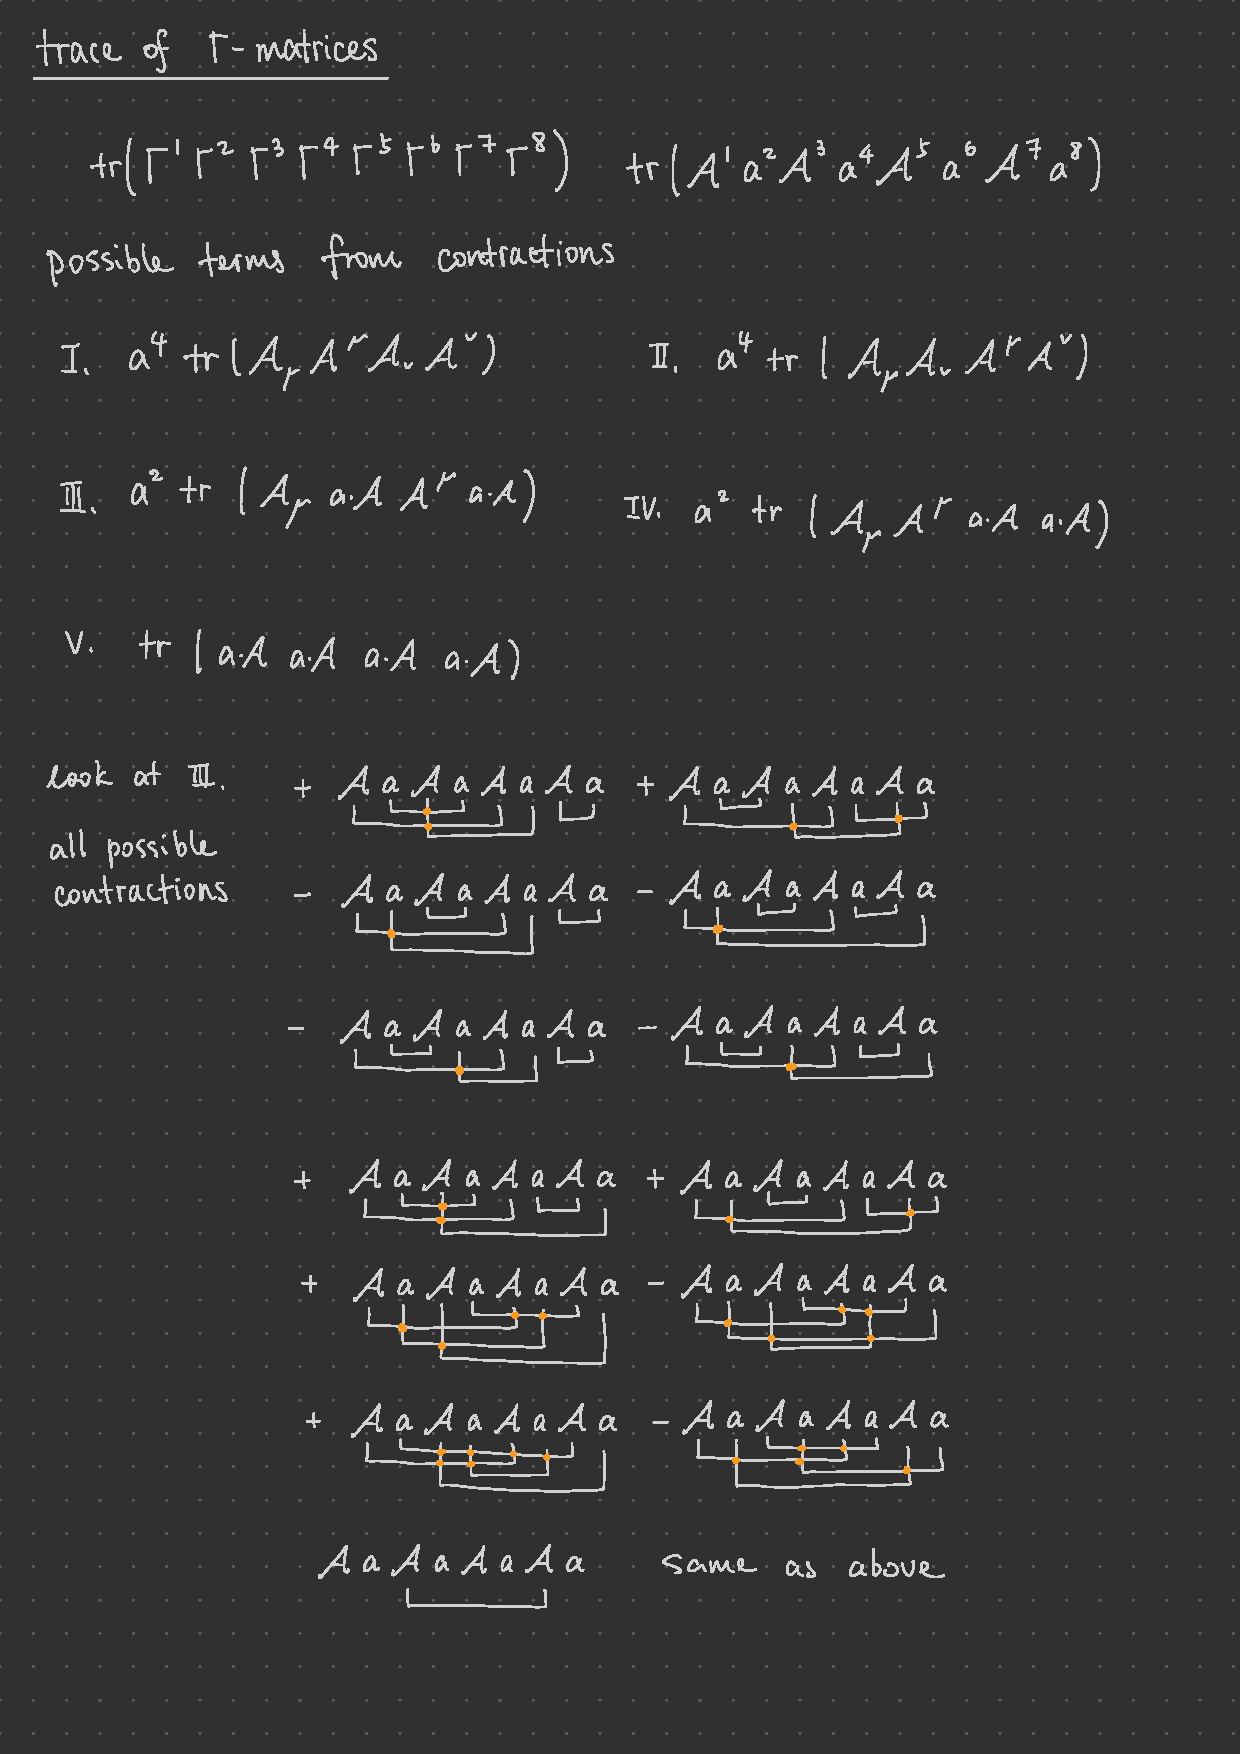
\includepdf{2024-04-24/notes-a.pdf}

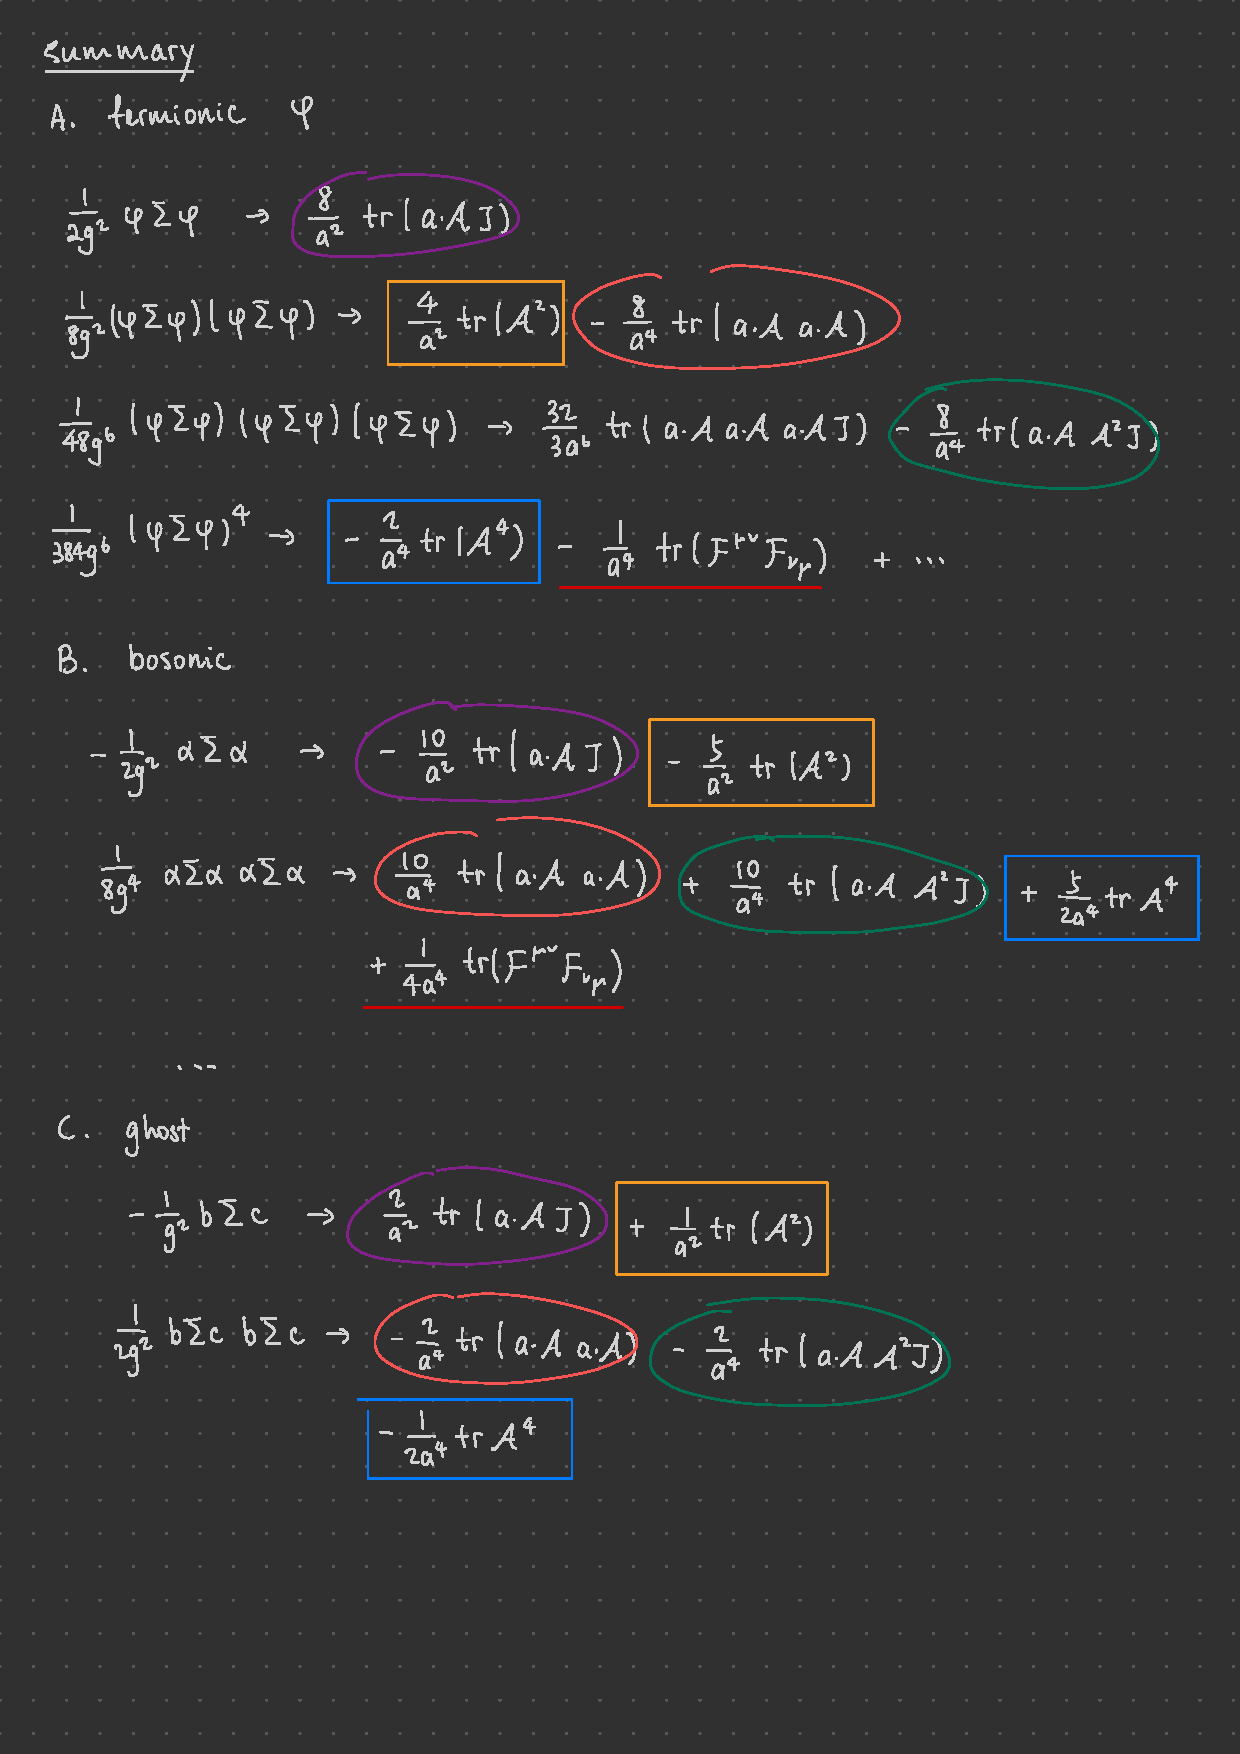
\includepdf{2024-04-24/notes-b.pdf}

\newpage

\paragraph{conceptual discussion of renormalization}
The basic question asked by the RG flow is:
how does the theory change with scale.

Scale is assumed as a part of definition of a theory.
The number of degrees of freedom depends on the scale.
Physically, we only have access to a part of dof,
but assuming there are more.
That is to say: the definition scale $\Lambda$ (cut-off)
is larger than the observational scale $\mu$.
What we are really asking is \emph{not} how the theory depending
on the $\Lambda$,
\emph{but} how the theory depending on the $\mu$.

A theory in physics sometimes appears in the form of a path integral.
It's by natural a proability distribution of the assumed dof.
In this sense, an effective theory can be translated to a marginal pdf in math.
A marginal pdf can be very different from the original pdf:
we do not expect to write them in a similar form.
But Gaussian is an exception.
Then it seems reasonable to perturb the Gaussian,
and study the marginal pdf.

One problem is: certain perturb may generate other perturb in marginal.
So if the starting point is already taken as marginal,
the consistency requires to include those ``derived perturb''.
If there is an infinite amount of them...

\begin{problem}
	An assumption of the matrix RG: $\text{off diag. } \ll \text{diag.}$?
	This is an assumption for the perturbative calculation.
	I don't know how the formulate this approximation properly
	because the matrix integral in any case get contribution from
	all possible matrix configurations.
	We are restricting to a particular integration domain,
	which don't have a definite mathematical definition.
\end{problem}

\begin{problem}
	Look at this term from the expansion (although it vanishes due to cancellation)
	\[
	\frac{1}{a^2}\mathrm{Tr}A^2
	\] 
Assume that (as one can always do) $a$ is much larger than the diagonal elements of $A$.
(assume $A$ is diagonal dominates)
This means that
\[
	\frac{1}{a^2} \mathrm{Tr} A^2 \sim N^x,\quad x<1
\] 
because the number of diagonal entries of $A^2$ that is comparable to $a^2$ is smaller than $N$.
We need to compare it with $\frac{1}{g^2}\mathrm{Tr}A^2$.
However, there is no $a>A$ to normalize the elements of $A$ smaller than $1$.
We want this term is much larger than $\frac{1}{a^2}$ term whatever $A$ is.
Is it possible? Define $g^2 N = t$, so $\frac{N}{t}\mathrm{Tr}A^2$ dominates when $N\to\infty$.
Only in this limit, our calculation makes sense.
It's always confusing we are studying $N$-flow in $N\to\infty$ limit.
It maybe understood as $n$-flow: $n\equiv \frac{N}{N_0}$ in $N\to\infty,N_0\to\infty$ limit.
\end{problem}
